%%%%%%%%%%%%%%%%%%%%%%%%%%%%%%%%%%%%%%%%%%%%%%%%%%%%%%%%%%%%%%%%%%%%%%%%%%%%%%%%
\chapter{Conclusion and Future Work}
\label{ch:conclusion}
%%%%%%%%%%%%%%%%%%%%%%%%%%%%%%%%%%%%%%%%%%%%%%%%%%%%%%%%%%%%%%%%%%%%%%%%%%%%%%%%

\section{Future Work}

In this section we present some ideas for future works and implementation for SIMITAR. On the first section "Improoving results", we suggest approaches for improving the current results. They include calibration of some constants, finer controll of packet injection, and performance improovments. 

\subsection{Improoving results}

\subsubsection{Tool calibration}

To imprrove our results, one aproach can be a perform  a deeper study on how calibrate each tool, depending on themain porpose. It can be done first adjusting some parameters and constants of our algorithms and procedures, wich may affect the performance. Some parameters will change the performance  of the tools that support stochastic functions for inter pacekt times:

\begin{itemize}
	
	\item \texttt{DataProcessor::minimumAmountOfPackets}: we just estimate stochastic models for inter-packet times, if the number of flow packets is larger then it. If it is smaller, we just apply the constant model, because with a small sample, the acuracy of any model is poor. Today its value is set to 30.
	
	\item \texttt{DataProcessor::min\_time}: minimum time considered on inter packet times. This is used to avoid inter packet times equals to zero, due the sniffer resolution. This may change the fitting acuracy, wich may change the performance of tools wich use inter-packet time models. Today, this value is $5e-8$. 

\end{itemize}

Others parameters and change of approaches may change the performance for any type of underlying tools or API. They are:

\begin{itemize}

	\item \texttt{DataProcessor::m\_min\_on\_time}: this value controls the small ON time that a \textit{file} can have. This value we can change de precission of the generated traffic. Currently this value is $0.1$s. 
	
	\item \texttt{DataProcessor::m\_session\_cut\_time}:  this member is responsible for defining whaterver a file transfecence still active or has ended. It defines the minimum OFF timme acceptable.
	
	\item \textit{Control a minimum number of pacekts required for a flow be created}: This would reduce the number of flows created. Since each flow is menaged by a different thread, it can imporrove the performance, reducing overheads. This action should not heavely impact negativally on the throughtput and scalling characteristics, but can increase the precision of the most significant flows. This apply for all underlying traffic-gen engines.
	
	
\end{itemize}



Para extensão do trafego gerado, é necessário um estudo da melhor calibração para cada ferramente, como o D-ITG, Iperf, Libtins, o que pode melhorar os resultados

\subsubsection{SIMITAR as a Packet Injector}

This proposed functionality is still unther implementation, and we are using Libtins API\footnote{\href{http://libtins.github.io/}{http://libtins.github.io/}}. It enable packet crafting and injection at a reasonable performance, adn provide support for many protocols. It is not thread safe, so will require some cares, such as use of mutexes. But will enable a finer controll of packet header contents, packet size, inter packet times and number of pacekts sent. In that way, we expect to achieve better results.  



\begin{figure}[!ht]
	\centering
	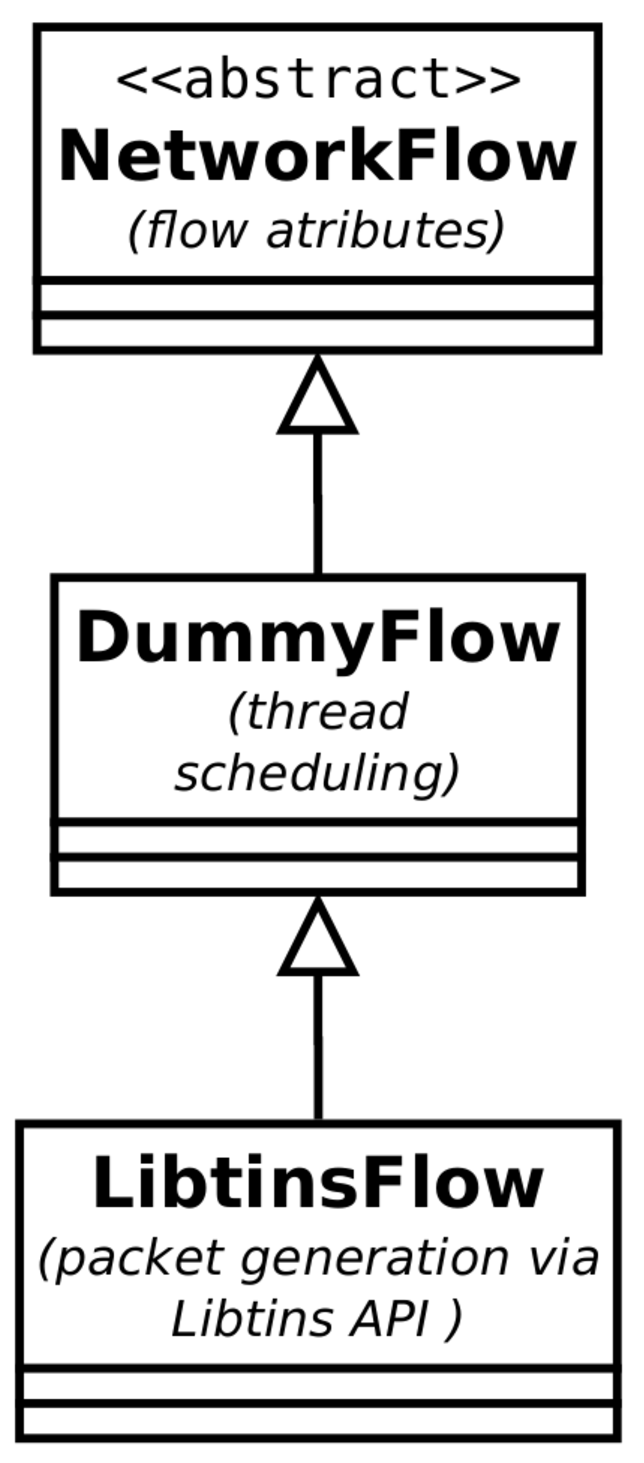
\includegraphics[height=2.0in]{figures/ch6/libtins-flow}
	\caption{Expansion of SIMITAR using Libtins for traffic generation}
	\label{fig:libtins-flow}
\end{figure}

\subsubsection{Traffic generation performance}


\begin{figure}[h!]
	\centering
	\subfloat[DpdkFlow]{
		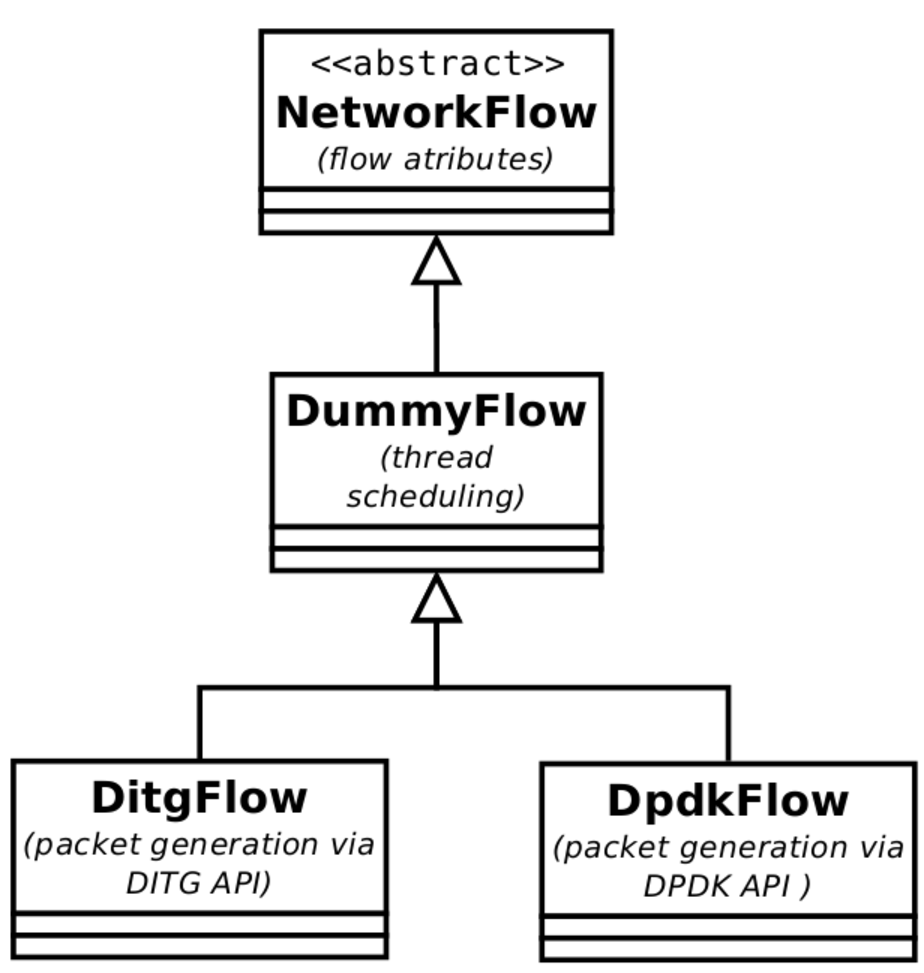
\includegraphics[height=2.0in]{figures/ch6/dpdk-flow}
		\label{fig:dpdk-flow}
	}
	\hspace{0mm}
	\subfloat[DpdkInterface]{
		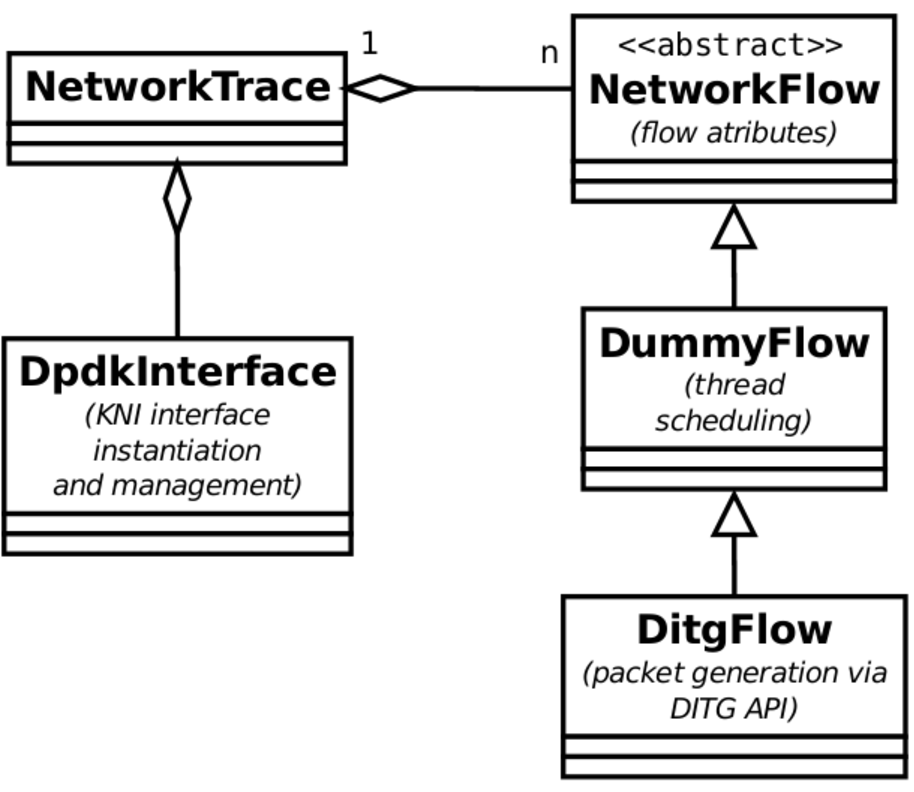
\includegraphics[height=2.0in]{figures/ch6/dpdk-interface}
		\label{fig:dpdk-if}
	}
	\caption{Class diagram for DPDK support expansions. On (a), we have a implementation of traffic generation based on DPDK. On (b) we are using DPDK KNI interfaces.}
	\label{fig:DpdkFlow}
\end{figure}

Some aproaches may be taken to improove the traffic generation performance. One possibility is use DPDK KNI interfaces \footnote{\href{http://dpdk.org/doc/guides/prog_guide/kernel_nic_interface.html}{http://dpdk.org/doc/guides/prog\_guide/kernel\_nic\_interface.html}}. The The DPDK Kernel NIC Interface (KNI) allow applications from the users apace interact with DPDK ports. In this way we may achieve a faster packet processing. 


Another poossibility is use DPDK API craft packets. Using a low level library such for packet generation, we will be able to custom generate packetes, and bypass the Linux network stack (packet acceleration). We present in the figure ~\ref{fig:DpdkFlow} how we could expand our tool to implement an packet generator based on DPDK.

\subsubsection{Thread Menager}

Instead of each flow thread controll individually each sleep and waken times, a better approach would be a separed thread controll and manage all the other thereads life-cycle operation.


\subsubsection{Improving DataProcessor Performance}

Melhorar os algoritimos adicionando técnicas adicionais de modelagem, como condição de parada para o algoritimo gradient descendent, stochastic gradient descendent, entre outros


\subsection{Further Implementations}


\begin{itemize}
	\item \textbf{C++ Sniffer}: Implementing the Sniffer and its SQL queries in C++ should increace its performance.
	
	\item \textbf{Use OpenDayLight REST API for data collection}: Another different approach for data collection ould be use the OpenDayLight REST API to collect data from a SDN OpenFlow switch, instead of a Sniffer. Using the REST API it is possible to stract many statistics from nodes, hosts and ports, such active flows, number of packets matched per flows, packet dopeds, and so on. But, in this case, different featutres would be measured, what would require a development of a new model for traffic generation. On the other hand, many precedures could be reused. 
	
	\item \textbf{SIMITAR Python API}: Currently, SIMITAR only enable the programming of flow traffic generation in C++. Adding Python support for reading NetwrokTrace and NetworkFlow objects would enalbe an easy expantion using Python traffic generation API, without the  need for creating "C++" wrappers.
	
	\item \textbf{Expand SIMITAR}: Expand the SIMITAR support for many other traffic generator tools and APIs, such as MoonGen LUA API, Ostinato Python API, Seagull traffic generator, and many others.
	
		\begin{figure}[!ht]
			\centering
			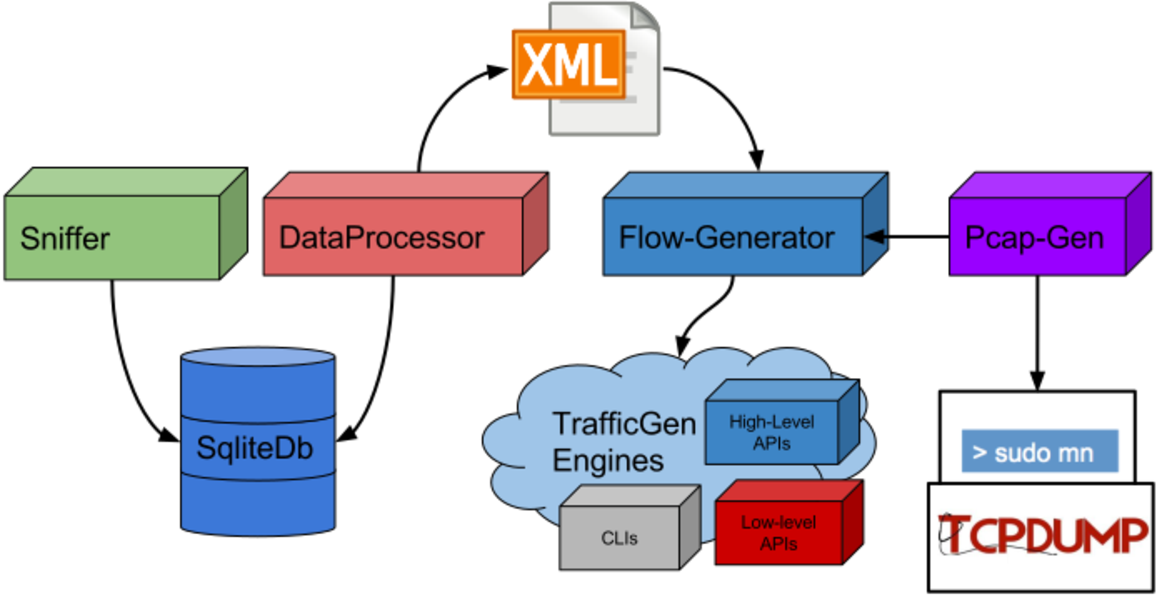
\includegraphics[height=2.0in]{figures/ch6/pcap-gen}
			\caption{Using SIMITAR for generation synthetic \textit{pcap} files, CTD files: a component schema}
			\label{fig:pcap-gen}
		\end{figure}
	
	\item \textbf{PcapGen: a compact \textit{pcap} lybrary}: This idea reffers to create a component capable of generate synthetic \textit{pcap} files, using Compact Trace Descriptors. This can be implemented using SIMITAR as a packet injector, but in an emulated host interface, using Mininet. Then, the traffic could be collected, using a tool such as TCPDump or Tshark. We present a diagram of this idea in the figure ~\ref{fig:pcap-gen}. This would enable SIMITAR works as trace lybrary for pcap-based benchmark tools.
	

	
	% Oferecer a possibilidade de automatização de medições e testes extendendo a ferramenta
	
	% usar redes neurais para classificação de aplicações
	
\end{itemize}










